\section{Résultats}

\paragraph{Étalonnage des transformateurs}
Les cycles à vide des transformateurs permettent de trouver \(\alpha\) tel que \(V_f = \alpha V_i\). Une régression linéaire sur le cycle du transformateur PHYWE à la \autoref{fig:phywe_vide} permet d'obtenir \mbox{\(V_f = (6.9 \pm 0.3)\times 10^{-2} V_i\)}. Une régression linéaire sur le cycle du transformateur cylindrique à la \autoref{fig:cylindre_vide} donne \mbox{\(V_f = (1.91 \pm 0.01)\times 10^{-2} V_i\)}. Pour ces régressions linéaires, l'ordonnée à l'origine a été négligée car elle était de l'ordre de \(10^{-4}\). Les erreurs ne sont pas représentées ici, mais le calcul d'erreurs se trouve en \autoref{sec:erreurs}. Le transformateur cylindrique ne présente pas d'hystérèse à vide, alors que le transformateur PHYWE possède une légère hystérèse, cependant la courbe reste linéaire sur la majorité du graphique.

\begin{figure}[h]
    \centering
    \begin{subfigure}{0.5\linewidth}
        \centering
        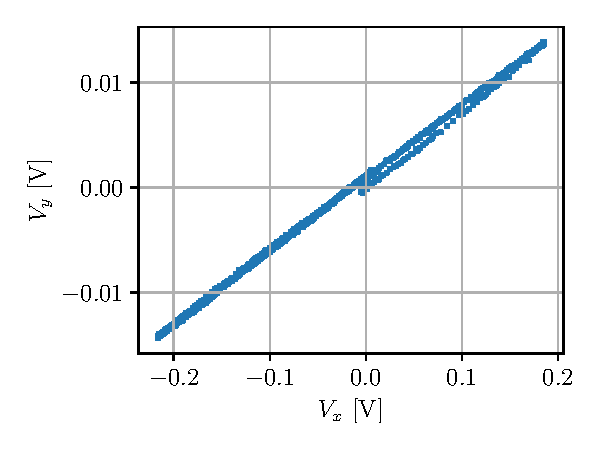
\includegraphics[width=\linewidth]{figures/G1-phywe-vide.pdf}
        \caption{}
        \label{fig:phywe_vide}
    \end{subfigure}%
    \begin{subfigure}{0.5\linewidth}
        \centering
        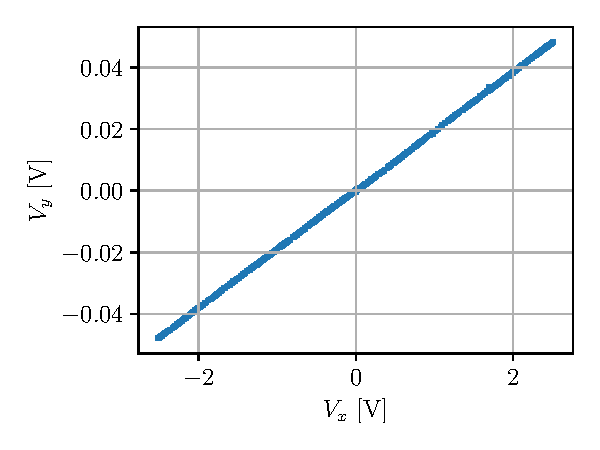
\includegraphics[width=\linewidth]{figures/G1-cylindre-vide.pdf}
        \caption{}
        \label{fig:cylindre_vide}
    \end{subfigure}
    \caption{Cycles à vide sur les transformateur (a) PHYWE (b) cylindrique}
\end{figure}

\paragraph{Propriétés des matériaux}
Les valeurs de \(\mu_r\) pour les différents échantillons étudiés ont été obtenues par l'\autoref{eq:mu_r} à l'aide des régressions linéaires sur les transformateurs à vide et sur les parties linéaires des graphiques des différents matériaux. Pour les matériaux diamagnétiques et paramagnétiques présentant un comportement purement linéaire cela représente l'entièreté des points relevés. Pour ceux présentant un cycle d'hystérèse seule la partie linéaire aux extremités du graphe a été utilisée pour la régression. La classification obtenue avec les valeurs des \(\mu_r\) est présentée dans le \autoref{tab:mu_r}.

\begin{table}[h]
    \vspace{5pt}
    \centering
    \begin{adjustbox}{width=\textwidth}
        \begin{tabulary}{\linewidth}{|c c c c c c c|}
            \toprule
            & Acier doux & Aluminium & Cuivre & Acier-Ag-Cr & Nickel-200 & Laiton \\
            \midrule
            \(\mu_r\) pour PHYWE & \(1.16 \pm 0.04\) & \(1.08 \pm 0.01\) & \(1.08 \pm 0.01\) & - & - & - \\
            \(\mu_r\) pour Cylindre & \(2.48 \pm 0.08\) & \(0.99 \pm 0.01\) & \(0.98 \pm 0.01\) & \(2.1 \pm 0.1\) & \(1.11 \pm 0.01\) & \(1.008 \pm 0.004\) \\
            Magnétisme & Ferro- & - & - & Ferro- & Ferro- & Para- \\
            \bottomrule
        \end{tabulary}
    \end{adjustbox}
    \caption{Valeurs de \(\mu_r\) pour différents échantillons dans chaque transformateur et leurs types de magnétisme (Ferro-, Para- et Dia- magnétisme)}
    \label{tab:mu_r}
\end{table}

\paragraph{Callibration des axes}
A partir des équations \autoref{eq:calibr_H} et \autoref{eq:calibr_B} il est possible de calculer les constantes pour pouvoir changer de variables et obtenir une induction magnétique en fonction d'un champ magnétique. En prenant pour le transformateur PHYWE \mbox{\(L = 6.4 \pm 0.1\) \si{\centi \meter}} et \mbox{\(N = 600\)} le nombre de spires du primaire, les coefficients obtenus lorsque le bloc PHYWE est utilisé sont: \mbox{\(H = (4.6\pm0.1)\times10^3 V_i\)} et \mbox{\(B = (8.3\pm0.2)\times10^{-2} V_f\)}. La figure avec les axes calibrés est visible en \autoref{fig:calibr_phywe}. La même stratégie peut être appliquée à des cycles d'hystérèse différents, visibles à la \autoref{fig:autres_cycles} en \autoref{sec:resultats_bonus}.

\begin{minipage}{\linewidth}
    \begin{wrapfigure}{R}{0.5\linewidth}
        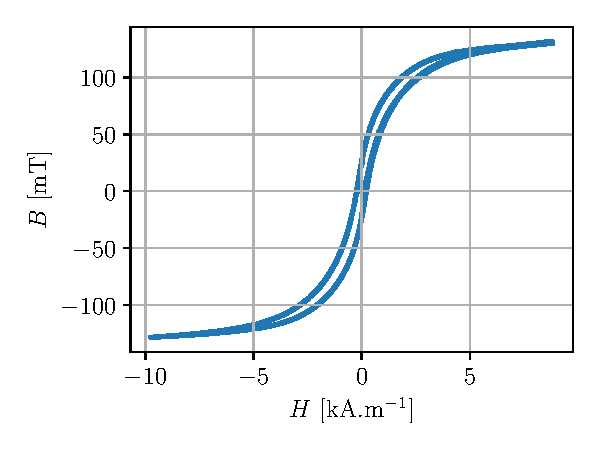
\includegraphics[width=\linewidth]{figures/G1-phywe-avec-bloc_chang.pdf}
        \caption{Cycle d'hystérèse du bloc PHYWE}
        \label{fig:calibr_phywe}
    \end{wrapfigure}

    Ces nouveaux graphiques permettent de mieux visualiser le système physique et les caractéristiques principales de son hystérèse à savoir les valeurs des \(H_c\), \(H_S\), \(B_r\) et \(B_S\). Pour le bloc PHYWE la valeur du champ coercitif après saturation est donc très proche de 0 \si{\kilo\ampere\per\meter}. Les valeurs de saturation  du champ magnétique et de l'induction respectivement peuvent être lues dans l'ordre de grandeur de 10 \si{\kilo\ampere\per\meter} et 200 \si{\milli\tesla}.

    \paragraph{Échantillons empilés}
    La \autoref{fig:combo} est obtenue en empilant deux échantillons du même matériau. Les épaisseurs des échantillons sont dans le \autoref{tab:thiccness} en \autoref{sec:resultats_bonus}. Pour les matériaux ferromagnétiques comme l'acier à la \autoref{fig:acier_combo}, la tension de sortie est presque doublée entre une simple et une double couche. Leur réponse au champ magnétique varie donc en fonction de l'épaisseur du matériau. Cependant, les autres échantillons, comme l'aluminium à la \autoref{fig:alu_combo} ne réagissent pas différement si l'épaisseur est changée.
\end{minipage}


\begin{figure}[h]
    \centering
    \begin{subfigure}{0.5\linewidth}
        \centering
        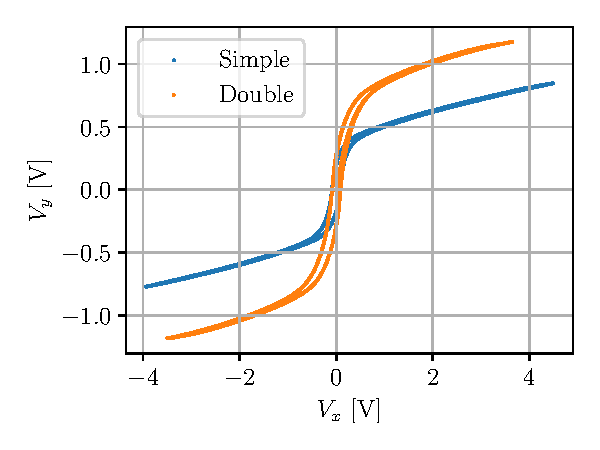
\includegraphics[width=\linewidth]{figures/ac_doux_simple_vs_combo.pdf}
        \caption{}
        \label{fig:acier_combo}
    \end{subfigure}%
    \begin{subfigure}{0.5\linewidth}
        \centering
        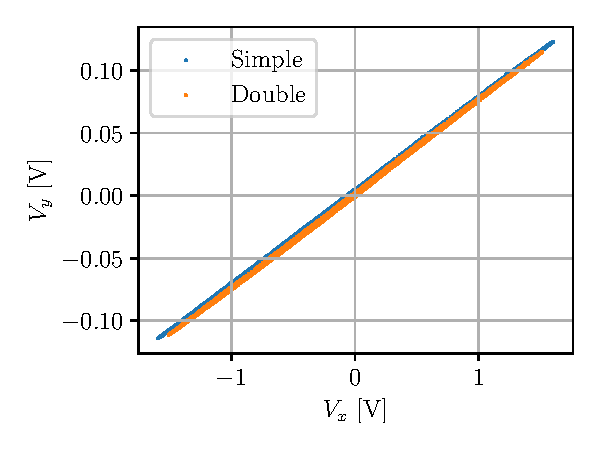
\includegraphics[width=\linewidth]{figures/alu_simple_vs_combo.pdf}
        \caption{}
        \label{fig:alu_combo}
    \end{subfigure}
    \caption{Comportement d'une simple et double couche pour des échantillons en (a) acier doux (b) aluminium}
    \label{fig:combo}
\end{figure}

\begin{wrapfigure}{R}{0.52\linewidth}
    \centering
    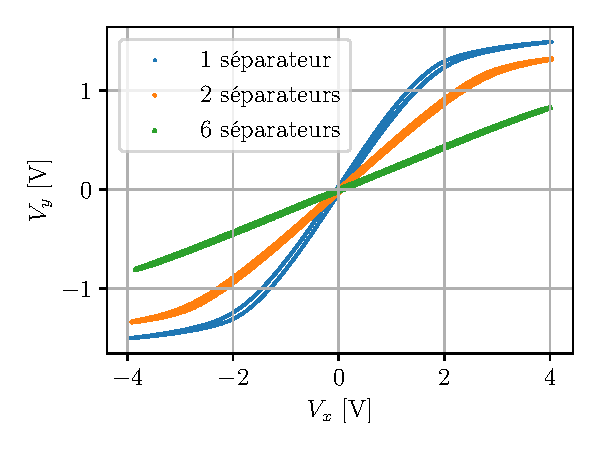
\includegraphics[width=\linewidth]{figures/separateurs_amagnetique.pdf}
    \caption{Réponse du bloc PHYWE après insertion de 1, 2 et 6 séparateurs amagnétiques}
    \label{fig:amagnetique}
\end{wrapfigure}

\paragraph{Plaques amagnétiques}
L'insertion de plaques amagnetique entre le transformateur et le bloc PHYWE change aussi la réponse du bloc, comme le montre la \autoref{fig:amagnetique}. Un nombre plus grand, correspondant à une plus grande épaisseur, de plaques amagnétiques diminue et même élimine le cycle d'hystérèse du bloc, qui répond alors linéairement au changement de champ magnétique.

% \paragraph{Orientation du bloc PHYWE}
% Le bloc PHYWE est composé de plusieurs couches de fer \cite{bloc_phywe}. La \autoref{fig:orientation_bloc} donne la réponse du bloc PHYWE en fonction de l'orientation des lamelles. Lorsque les lamelles sont orientées dans un sens différent que prévu, ici verticalement, le champ magnétique est moins fort que pour l'orientation prévue, avec les lamelles horizontales.

% \begin{figure}[h]
%     \begin{minipage}{0.48\linewidth}
%         \centering
%         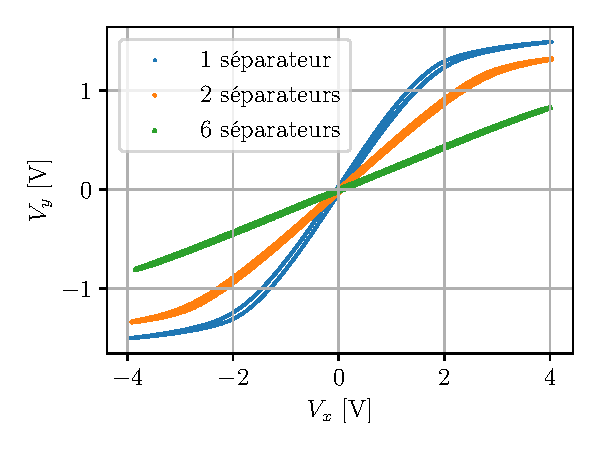
\includegraphics[width=\linewidth]{figures/separateurs_amagnetique.pdf}
%         \caption{Réponse du bloc PHYWE après insertion de 1, 2 et 6 séparateurs amagnétiques}
%         \label{fig:amagnetique}
%     \end{minipage}
%     \hfill
%     \begin{minipage}{0.48\linewidth}
%         \centering
%         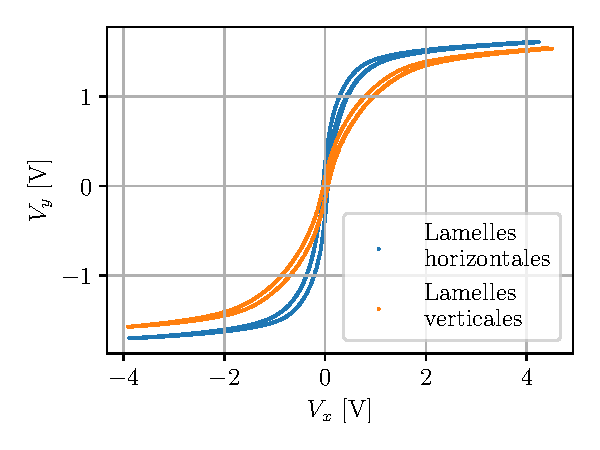
\includegraphics[width=\linewidth]{figures/vertical_vs_horizontal.pdf}
%         \caption{Comportement du bloc PHYWE en fonction de l'orientation des lamelles}
%         \label{fig:orientation_bloc}
%     \end{minipage}
% \end{figure}
    
